%%%%%%%%%%%%%%%%%%%%%%%%%%%%%%%%%%%%%%%%%%%%%%%%%%%%%%%%%%%%
\documentclass[a4paper,11pt,oneside]{article}
\usepackage[a4paper,vmargin={1.cm,2.5cm},width=19cm,]{geometry}
\usepackage[style=verbose-inote,doi=false,sortcites=true,block=space,backend=bibtex]{biblatex}
\usepackage[utf8]{inputenc}
\usepackage{textcomp}
\usepackage[spanish]{babel}
\usepackage{microtype}
\usepackage{lmodern}
\usepackage{graphicx}
\usepackage{fancyhdr}
\usepackage{booktabs}
\usepackage{eurosym}
\usepackage{mathptmx}
\usepackage[T1]{fontenc}
\usepackage{hyperref}
%% Added to help mimic structure.
\usepackage{tcolorbox}
\tcbuselibrary{breakable}
\usepackage{soul}
\usepackage{color}
\usepackage{multirow}
\usepackage{xcolor,colortbl}
\usepackage{tabularx}
\usepackage{tikz}

\setlength{\headheight}{1cm}
\setlength{\headsep}{0.5cm}
\pagestyle{fancy}
\fancyheadoffset[HR,HL]{2cm}
\fancyfootoffset[HR,HL]{2cm}
\fancyhf{}
\lfoot{\hspace{2cm}{\scriptsize CONSELLERA DE EDUCACI\'O, INVESTIGACI\'O, CULTURA I ESPORT. DIRECCI\'O GENERAL DE UNIVERSITAT, INVESTIGACI\'O I CI\`ENCIA}\\\hspace{2cm}{\scriptsize CONSELLERIA DE EDUCACI\'ON, INVESTIGACI\'ON, CULTURA Y DEPORTE. DIRECCI\'ON GENERAL DE UNIVERSIDAD, INVESTIGACI\'ON Y CIENCIA}}
%\cfoot{testtest}
\renewcommand{\headrulewidth}{0pt} % remove lines
%\renewcommand{\footrulewidth}{0pt}

%%%%%%%%%%%%%%%%%%%%%%%%%%%%%%%%%%%%%%%%%%%%%%%%%%%%%%%%%%%%
%% Hack to make math formulas bold in section titles
\makeatletter
\DeclareRobustCommand*{\bfseries}{%
  \not@math@alphabet\bfseries\mathbf
  \fontseries\bfdefault\selectfont
  \boldmath
}
\makeatother

%%%%%%%%%%%%%%%%%%%%%%%%%%%%%%%%%%%%%%%%%%%%%%%%%%%%%%%%%%%%
\def\thesection{\bf \textsf{\alph{section}}}

%% Special box for figures.
\newtcbox[auto counter]{\figbox}[2][]{
  colback=white,colframe=gray,colbacktitle=white,coltitle=black,title=Figure~\thetcbcounter: #2,#1
}

\begin{document}
%%%%%%%%%%%%%%%%%%%%%%%%%%%%%%%%%%%%%%%%%%%%%%%%%%
% $Id: commands.tex 1931 2015-01-17 10:32:50Z jmalbos $
% Some useful new commands...

%%%%%%%%%%%%%%%%%%%%%%%%%%%%%%%%%%%%%%%%%%%%%%%%%%
% BB
\newcommand{\bb}{\ensuremath{\beta\beta}}
% BB0NU
\newcommand{\bbonu}{\ensuremath{0\nu\beta\beta}}
% BB2NU
\newcommand{\bbtnu}{\ensuremath{2\nu\beta\beta}}

%%%%%%%%%%%%%%%%%%%%%%%%%%%%%%%%%%%%%%%%%%%%%%%%%%
% mBB
\newcommand{\mbb}{\ensuremath{m_{\bb}}}
% T0nu
\newcommand{\Tonu}{\ensuremath{T_{1/2}^{0\nu}}}

\newcommand{\tto}{\ensuremath{t_0}}

% Gonu
\newcommand{\Gonu}{\ensuremath{G^{0\nu}}}
% MNE
\newcommand{\Monu}{\ensuremath{\left|M^{0\nu}\right|}}
% Qbb
\newcommand{\Qbb}{\ensuremath{Q_{\bb}}}

%%%%%%%%%%%%%%%%%%%%%%%%%%%%%%%%%%%%%%%%%%%%%%%%%%
% kg·year
\newcommand{\kgy}{\ensuremath{\mathrm{kg}\cdot\mathrm{yr}}}
% Mbb
\newcommand{\Mbb}{\ensuremath{M_{\bb}}}
% kgbb
\newcommand{\kgbb}{\ensuremath{\mathrm{kg}_{\bb}}}
% ckky
\newcommand{\ckky}{\ensuremath{\mathrm{cts~keV^{-1}~kg^{-1}~yr^{-1}}}}
% ckkbby TO BE REVISED
\newcommand{\ckkbby}{\ckky}

%%%%%%%%%%%%%%%%%%%%%%%%%%%%%%%%%%%%%%%%%%%%%%%%%%
% Ca-48
\newcommand{\CA}{\ensuremath{^{48}\mathrm{Ca}}}
% Ge-76
\newcommand{\GE}{\ensuremath{^{76}\mathrm{Ge}}}
% Se-82
\newcommand{\SE}{\ensuremath{^{82}\mathrm{Se}}}
% Zr-96
\newcommand{\ZR}{\ensuremath{^{96}\mathrm{Zr}}}
% Mo-100
\newcommand{\MO}{\ensuremath{^{100}\mathrm{Mo}}}
% Pd-110
\newcommand{\PD}{\ensuremath{^{110}\mathrm{Pd}}}
% Cd-116
\newcommand{\CD}{\ensuremath{^{116}\mathrm{Cd}}}
% Sn-124
\newcommand{\SN}{\ensuremath{^{124}\mathrm{Sn}}}
% Te-130
\newcommand{\TE}{\ensuremath{^{130}\mathrm{Te}}}
% Xe-136
\newcommand{\XE}{\ensuremath{^{136}\mathrm{Xe}}}
% Nd-150
\newcommand{\ND}{\ensuremath{^{150}\mathrm{Nd}}}

% Ba-136
\newcommand{\BA}{\ensuremath{^{136}\mathrm{Ba}}}

% Tl-208
\newcommand{\TL}{\ensuremath{^{208}\mathrm{Tl}}}
% Bi-214
\newcommand{\BI}{\ensuremath{^{214}\mathrm{Bi}}}

\newcommand{\URANIUM}{Uranium}
\newcommand{\THORIUM}{Thorium}

% Xe-136
\newcommand{\NA}{\ensuremath{^{22}}Na}
\newcommand{\CS}{\ensuremath{^{137}}Cs}



%%%%%%%%%%%%%%%%%%%%%%%%%%%%%%%%%%%%%%%%%%%%%%%%%%
% W-values
\newcommand{\Wi}{\ensuremath{W_\mathrm{i}}}
\newcommand{\Wsc}{\ensuremath{W_\mathrm{sc}}}




%%%%%%%%%%%%%%%%%%%%%%%%%%%%%%%%%%%%%%%%%%%%%%%%%%

\begin{tcolorbox}[colback=white,coltitle=black,arc=0pt,outer arc=0pt,colframe=black,boxrule=0.6pt,boxsep=0pt,left=0pt,top=0pt,right=0pt]
\begin{tabularx}{\textwidth}{@{}l|*1{>{\centering\arraybackslash}X}@{}}
  \hline
\raisebox{\dimexpr\ht\strutbox-\height\relax}{
\includegraphics[width=6cm,keepaspectratio=true]{img/logo_generalitat}} & {\small {\bf SOL·LICITUD D’AJUDES PER A LA REALITZACI\'O DE PROJECTES D’I+D PER A GRUPS D’INVESTIGACI\'O D'EXCEL·L\`ENCIA (PROMETEU 2016) SOLICITUD DE AYUDAS PARA LA REALIZACI\'ON DE PROYECTOS DE I+D PARA GRUPOS DE INVESTIGACI\'ON DE EXCELENCIA (PROMETEO 2016)}}\\
\hline
\end{tabularx}

\begin{tabularx}{\textwidth}{l X}
  \cellcolor{gray} {\bf A } &{\small {\bf MEM\`ORIA CIENTIFICOT\`ECNICA DEL PROJECTE/ MEMORIA CIENT\'IFICO-T\'ECNICA DEL PROYECTO}}\\
\hline
\end{tabularx}

\begin{tabularx}{\textwidth}{l X}
INVESTIGADOR RESPONSABLE DEL PROJECTE  / INVESTIGADOR RESPONSABLE DEL PROYECTO &\\
Juan Jos\'e G\'omez Cadenas &\\
& \\
\hline


T\'ITOL DEL PROJECTE / T\'ITULO DEL PROYECTO & \\
Desarrollo de nuevas tecnolog\'ias basadas en el Xen\'on para Ciencia B\'asica y Aplicada & \\
& \\
& \\
\hline

RESUM DEL PROJECTE / RESUMEN DEL PROYECTO & \\
\end{tabularx}

~Durante la última década, los miembros del grupo de investigación integrados en esta propuesta han liderado el desarrollo de nuevas tecnologías para la detección de radiación ionizante basadas en cámaras de gas xenón. Concretamente, el investigador principal (IP) propuso en 2007 el desarrollo de un nuevo tipo de detector llamado NEXT, una cámara de proyección temporal utilizado xenón a alta presión con amplificación electroluminescente de la señal. El principio básico de operación de este detector explota el rápido centelleo con que el xenón responde al paso de la radiación, así como sus propiedades de gas noble para medir la energía y trayectoria de partículas cargadas. Durante los años 2008 a 2014 el IP  ha liderado una colaboración internacional (colaboración NEXT) cuyo objetivo es la construcción de un detector con una masa de 100 kg de xenón enriquecido al 90\% en el isótopo \XE. El objetivo de este detector, cuya primera fase está siendo puesta a punto en el laboratorio subterráneo de Canfranc (LSC) es detectar un tipo de desintegración extremadamente raro del Xe-136, llamado desintegración doble beta sin neutrinos. La observación de dichos procesos supondría la demostración de que el neutrino es su propia antipartícula, un descubrimiento con profundas consecuencias en física de partículas y cosmología, que tendría una relevancia comparable al descubrimiento de las oscilaciones de neutrinos o del bosón de Higgs (hallazgos que ha sido galardonados con un premio Nobel). El desarrollo de NEXT fue financiado hasta 2014 por proyectos del MICYNT/MINECO así como por un proyecto CONSOLIDER-INGENIO 2010 y ha obtenido en 2014 un prestigioso Advanced Grant/ERC. 

~Por otra parte, durante el año 2015, el IP de este proyecto ha propuesto la aplicación de la tecnología desarrollada para NEXT a un nuevo tipo de detector PET para imagen médica, basado en el xenón líquido llamado PETALO. Este detector presenta dos grandes ventajas sobre los centelladores sólidos convencionales (tales como LSO). Por un lado es mucho más económico, lo que permitiría desarrollar aparatos PET de gran sensibilidad a bajo coste. Por otro, el tiempo de respuesta en centelleo es mucho más rápido lo que permite una medida de tiempo de vuelo (TOF) excepcionalmente buena (con una resolución temporal de 100 ps o menos), lo que a su vez contribuye a una reducción espectacular de los ruidos de fondo característicos de la tecnología (coincidencias accidentales, dispersión Compton, etc.). La tecnología de PETALO, que ha sido protegida por una patente de la cual la UV es co-propietaria junto al CSIC podría suponer una desarrollo extremadamente innovador en la tecnología PET.
 

{\bf ~El primer objetivo de este proyecto de investigación} es contribuir al desarrollo de NEXT, que podría ser el primer experimento de física de partículas realizado en España capaz de realizar o contribuir a un descubrimiento fundamental. 

{\bf ~El segundo objetivo de este proyecto de investigación} es contribuir de manera decisiva al desarrollo del proyecto PETALO, realizando una serie de medidas fundamentales para demostrar la viabilidad de la tecnología y su potencial para la construcción de aparatos clínicos. 

\end{tcolorbox}

\newpage

\begin{tcolorbox}[breakable,colback=white,coltitle=black,arc=0pt,outer arc=0pt,colframe=black,boxrule=0.6pt,boxsep=0pt,left=0pt,top=0pt,right=0pt]

\begin{tabularx}{\textwidth}{X}
\\
\\
\\
\\
\\
\hline
\end{tabularx}



{\bf
Mem\`oria cientificot\`ecnica i pressupost del projecte d’investigació per a tota la durada del projecte, distribu\"it per anualitats. \\ Memoria cient\'ifico-t\'ecnica del proyecto de investigaci\'on para toda la duraci\'on del proyecto, distribuido por anualidades.
}


\section*{Proyecto NEXT}

\subsection*{Neutrinos de Majorana}
Una de las preguntas más importantes que se plantea la física de partículas moderna es la de si el neutrino es su propia antipartícula, tal como fue postulado por el físico italiano Ettore Majorana, alrededor de 1930. La importancia de esta cuestión radica en la necesidad, por parte de las teorías de leptogénesis, de introducir neutrinos de Majorana como un ingrediente esencial para generar la asimetría cósmica entre materia y antimateria. La presencia de neutrinos de Majorana pesados también permitiría explicar el hecho de que las masas de los neutrinos ligeros sea mucho más pequeña que la de los correspondientes leptones. 

La desintegración doble beta (\bb) es un proceso débil de segundo orden en el que un núcleo con número atómico Z y masa atómica A se transforma en su isóbaro con número atómico 
Z+2:

\begin{equation}
(Z,A) \rightarrow (Z+2,A) + 2 e^- + 2 \bar{\nu}_e 
\end{equation}
%                                     
Los procesos \bb\ han sido observados en numerosos isótopos, midiéndose vidas medias en el rango de $10^{18} - 10^{21}$ años. Se trata del proceso de desintegración radioactiva más lento que se conoce. Sólo se observa en 35 isótopos naturales, en los que la desintegración beta convencional al núcleo (Z+1) está suprimida o prohibida energéticamente. 

Por otra parte la desintegración doble beta sin neutrinos (\bbonu):
                                     
\begin{equation}
(Z,A) \rightarrow (Z+2,A) + 2 e^- 
\end{equation}
 %                                    
sólo puede darse si los neutrinos son partículas de Majorana. El mecanismo más sencillo para producir esta desintegración implica el intercambio de neutrinos ligeros y viene caracterizado por una vida media \Tonu\ cuya inversa es proporcional al cuadrado de la llamada masa efectiva de Majorana, \mbb: 
                                    
\begin{equation}
(\Tonu)^{-1} =\Gonu \Monu^2 \mbb^2 ,
\label{eq.t0nu}
\end{equation}
%  
donde el término \Gonu\ es un factor de espacio de fases y el término \Monu\ un elemento de matriz nuclear. La masa  de Majorana, \mbb\ , es una superposición de los tres autoestados de masa de los neutrinos, ${\rm m_i ~(i=1,3)} $: 
                                    
\begin{equation}
\mbb =|m_1 |U_{e1}|^2 + m_2 |U_{e2}|^2 e^{i\alpha}+ m_3 |U_{e3}|^2 e^{i\beta}| ,
\label{eq.mbb}
\end{equation}
%
donde los factores $U_{ei}$~ son elementos de la matriz de mezcla leptónica y $\alpha,\beta$ son las llamadas fases de Majorana. Así pues, el periodo de la desintegración \bbonu\ aumenta a medida que la masa de Majorana se hace más y más ligera. Los límites actuales en el periodo \Tonu\  (del orden de 10$^{25}$~ años) pueden traducirse en límites en la masa de \mbb\ (del orden de 130-300 meV). La considerable incertidumbre en dichos límites se debe a las dificultades teóricas para calcular el elemento de matriz nuclear \Monu.  

Desde el punto de vista experimental, la desintegración \bbonu\ ofrece una señal característica. En efecto, la ausencia de neutrinos se traduce en que la suma de las energías cinéticas de los dos electrones emitidos en el proceso es siempre la misma, e igual a \Qbb: 
                                    
\begin{equation}
\Qbb =M(A,Z) - M(A, Z+2)
\label{eq.mbb}
\end{equation}
%
Por tanto, para un experimento de \bbonu\ es importante medir con buena resolución  la energía de los dos electrones. En el límite de un detector de resolución perfecta, bastaría con observar una desintegración tal que la suma de las energías de los dos electrones fuera idéntica a \Qbb\  para establecer que se trata de una desintegración \bbonu. En la práctica, incluso los detectores con mejor resolución energética (basados en cristales semiconductores de germanio o bolómetros de telurio) miden una distribución de energía con una cierta anchura a media altura (FWHM) del orden de unos pocos keV. Por otra parte, las vidas medias del proceso \bbonu\ son muy largas. Teniendo en cuenta que los ruidos de fondo a este proceso están relacionados con las cadenas naturales del uranio y el torio, con vidas medias características de $10^{10}$~ años, nos encontramos con que los experimentos \bbonu\ deben reducir los potenciales ruidos de fondo en más de 15 órdenes de magnitud. 

\subsection*{El experimento NEXT}

Uno de los mejores isótopos para buscar procesos \bbonu\ es el \XE. El xenón es un gas noble, que permite construir aparatos que sean simultáneamente blanco y  detector, aprovechando las propiedades de centelleo e ionización del gas. En concreto, el experimento NEXT propone la construcción de cámaras de proyección temporal (TPCs) utilizando xenón a alta presión (HPXe) y amplificando la señal de ionización mediante electroluminescencia (EL). El gas xenón está enriquecido al 90\% en \XE. 


\begin{figure}
\centering
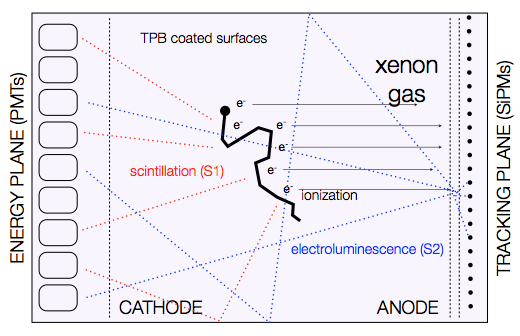
\includegraphics[width=0.8\textwidth]{img/EL.png}
\caption{\small Principio de operación del detector NEXT. 
} \label{fig.EL}
\end{figure}
                                    
El principio de operación de NEXT se ilustra en la Figura \ref{fig.EL}. Cuando se produce un suceso ionizante en el xenón (sea este una desintegración \bb\ o un suceso de ruido de fondo, por ejemplo la interacción Compton o fotoeléctrica de un fotón de alta energía) la respuesta del gas es la emisión de luz de centelleo ultravioleta (UV) con una longitud de onda cuyo pico se sitúa en 172 nm. Esta luz de centelleo es copiosa (del orden de 60,000 fotones por MeV de energía depositada) y, como se verá, constituye la base de funcionamiento de PETALO, descrito posteriormente en esta memoria. En el detector NEXT el centelleo primario permite medir el tiempo inicial (\tto) de la interacción.

Los electrones de ionización producidos por el paso de la radiación son arrastrados en el detector NEXT hacia el ánodo, merced a un campo eléctrico de unos 300 V/cm. Antes de llegar al ánodo, los electrones atraviesan una rejilla situada a un potencial de unos 15,000 voltios con respecto al ánodo. Como consecuencia, los electrones se aceleran, emitiendo del orden de 1,000 fotones ultravioleta durante el tiempo que necesitan para cruzar la llamada región de electroluminescencia. Estos fotones se emiten isotrópicamente. Los fotones que se propagan hacia el ánodo son registrados por un plano de detectores de estados sólido llamados fotomultiplicadores de silicio (SiPMs) situado detrás de este. Los fotones que se propagan en otras direcciones llegan hasta un plano de fotomultiplicadores convencionales (PMTs) situados tras el cátodo. El plano de SiPMs se llama plano de trazado y, permite reconstruir la trayectoria de los electrones primarios. El plano de PMTs se llama plano de energía y permite reconstruir la energía del evento. 

La tecnología de NEXT conjunta varias ventajas importantes para la realización óptima de un experimento \bbonu:
                                    
                                    %%%%%
\begin{figure}
\centering
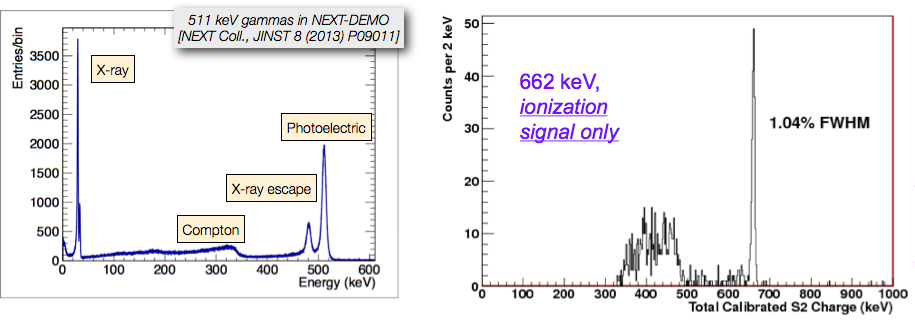
\includegraphics[width=0.9\textwidth]{img/EResolution.png}
\caption{\small Izquierda: Espectro de energía medido para electrones de 511 keV en el detector NEXT-DEMO. Derecha: El espectro cerca del pico fotoeléctrico a 662 keV. La resolución at 662 keV es 1\% FWHM, lo que extrapola a 0.5\% FWHM en \Qbb.}
\label{fig.ERES}. 
\end{figure}
%%%%

%%%%%
\begin{figure}
\centering
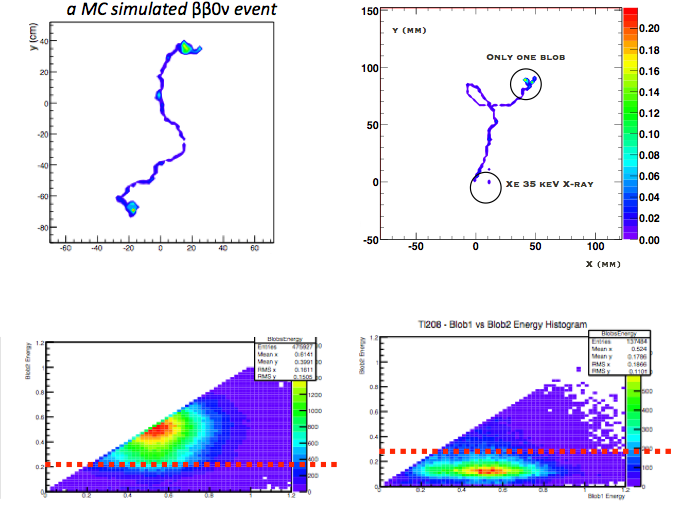
\includegraphics[width=0.9\textwidth]{img/Topo2.png}
\caption{\small NEXT es uno de los pocos experimentos de búsqueda \bbonu\ que puede proporcionar una señal topológica. El panel superior izquierdo muestra la reconstrucción de un suceso de señal (generado por Monte Carlo), que consiste en dos electrones producidos en un vértice común. El panel superior derecho muestra un evento de ruido de fondo, que consiste en un electrón emitido por los isótopos  \BI\ o \TL. En el caso de la señal, aparecen dos bolas de energía depositadas en los extremos de la traza, mientras que el ruido de fondo muestra sólo una bola. En los paneles inferiores se representa la energía de las dos bolas que se encuentran en los extremos de la traza. En el caso de la señal (panel inferior izquierdo) la energía de ambas bolas es alta y aproximadamente igual. En el caso del ruido de fondo (panel inferior derecho) la energía de una de las bolas es muy pequeña. Un simple corte, requiriendo que la energía de ambas bolas sea superior a 0.2 MeV, separa eficientemente la señal del ruido.}\label{fig.ETRK2}
\end{figure}
%%%%%

\begin{enumerate}
\item {\bf Excelente resolución en energía} (Figura \ref{fig.ERES}) medida por la colaboración NEXT usando los prototipos NEXT-DEMO y NEXT-DBDM, desarrollados en la fase de I+D+i del experimento . Se obtiene una resolución de 0.5 \% FWHM en la zona de interés cercana a \Qbb. La resolución en energía de NEXT es un factor 8 superior a la del experimento EXO, basado en una cámara de xenón líquido y superior en un factor 20 a la del experimento KamLAND-Zen, donde el gas se disuelve en centellador líquido. 
\item {\bf Caracterización de la señal mediante una señal topológica} (Figura \ref{fig.ETRK2}). NEXT puede reconstruir la señal de los dos electrones emitidos en una desintegración \bb\, distinguiéndolos de la señal que proporcionan los ruidos de fondo, constituidos mayoritariamente por un solo electrón.
\item {\bf Alta radiopureza en los materiales que constituyen el detector}, minimizando contaminaciones radioactivas (trazas de las cadenas de uranio y torio) que puedan enmascarar la señal \bbonu.
\item {\bf La tecnología puede escalarse fácilmente a altas masas}. Al tratarse de detector continuo (el xenón es a la vez blanco y detector), cada vez que se doblan las dimensiones longitudinales del aparato se multiplica su masa por un factor de, aproximadamente $2^3$, mientras que la superficie escala como $2^2$. Dado que la señal es proporcional a la masa del blanco y los ruidos de fondo son aproximadamente proporcionales a las superficies del detector (donde se depositan las trazas radioactivas que los originan), cada vez que se doblan las dimensiones del detector se mejora la señal sobre el ruido en un factor $2^3/2^2 = 2$. 
\end{enumerate}

La economía de escala que presenta la tecnología  ha permitido la construcción de una serie de detectores para establecer progresivamente la validez de la tecnología y entender el impacto de los ruidos de fondo. El primero de estos detectores, NEXT-DEMO, permitió desarrollar los aspectos tecnológicos, muy novedosos, de las HPXe-EL y demostró, con una masa de 1 kg, excelente resolución en energía, así como una robusta señal topológica. En la actualidad, el detector NEW, con una masa de 10 kg, está comenzando a operar en el LSC y medirá con precisión los ruidos de fondo ambientales esperados en el experimento. El detector NEXT-100, con una masa de 100 kg, empezará a operar en el LSC en 2018. 


\begin{figure}
\centering
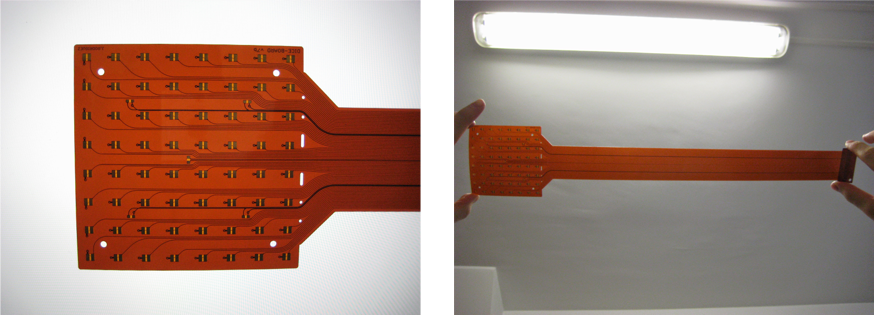
\includegraphics[width=0.9\textwidth]{img/KDB.png}
\caption{\small Los Kapton Dice Boards (KDB) de NEXT.} \label{fig.KDB}
\end{figure} 


Uno de los elementos más novedosos de NEXT es su plano de trazado que permite la reconstrucción de las trayectorias de los electrones en el gas. El plano de trazado está formado por matrices de SiPMs, organizadas en circuitos de kapton, llamados KDBs (de las siglas en inglés de Kapton Dice Boards). La Figura \ref{fig.KDB} muestra uno de estos KDBs, que suponen un diseño original de NEXT. El detector NEW cuenta con unos 25 KDBs, cada uno de los cuales tiene 64 SiPMs (1,600 canales en total). El detector NEXT-100 cuenta con 110 KDBs  (7040 canales).  

NEXT-100 podría descubrir la existencia de procesos \bbonu\ si su periodo es de hasta $10^{26}$~años. En caso contrario, la siguiente fase, denominada NEXT2N (next-to-next) contemplaría la construcción de un detector con una masa de centenares de kilos capaz de explorar periodos \Tonu\ del orden de $10^{27}$~años. {\bf En consecuencia, un experimento construido y en operación en España y liderado desde la Comunidad Valenciana, podría situarse al frente del campo de la física \bbonu\ en los próximos años}.
 
 
\begin{figure}
\centering
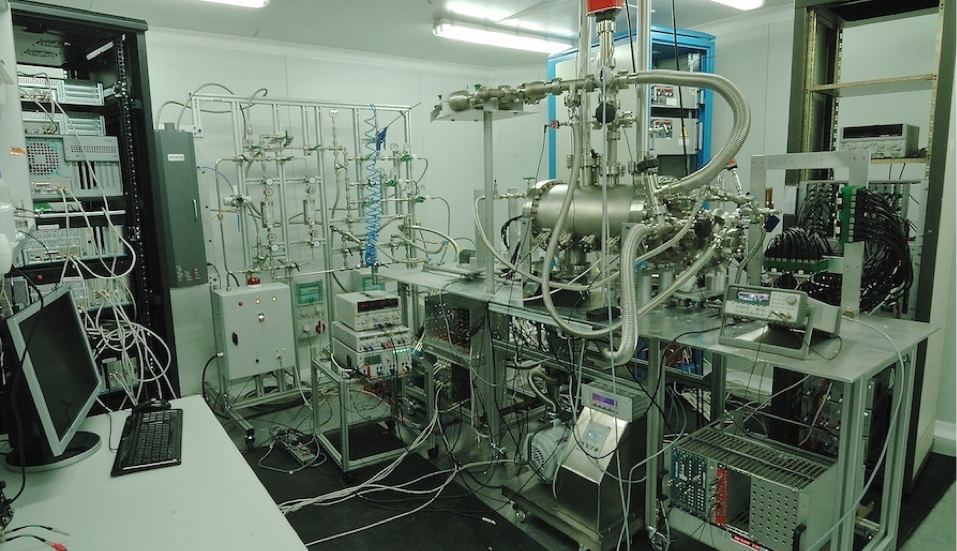
\includegraphics[width=0.9\textwidth]{img/DemoSetup.png}
\caption{\small El detector NEXT-DEMO en el laboratorio del IFIC (Valencia).} \label{fig.DEMO}
\end{figure}

%%%%%%%%%%
\begin{figure}
\centering
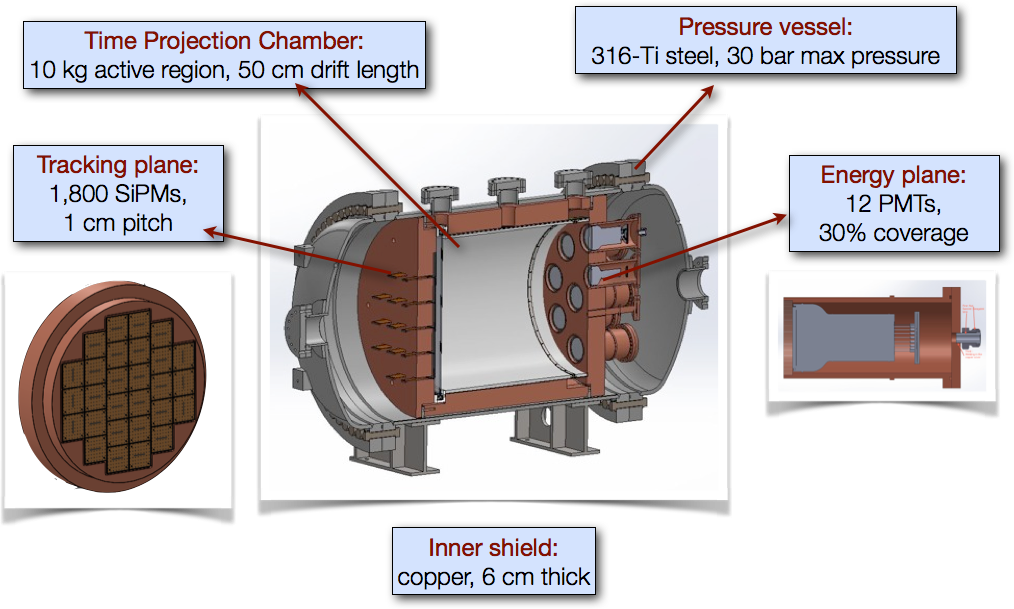
\includegraphics[width=0.9\textwidth]{img/NEW.png}
\caption{\small NEW, la primera fase del experimento NEXT en Canfranc.} \label{fig:NEW}
\end{figure} 

%%%%%%%%%%
\begin{figure}
\centering
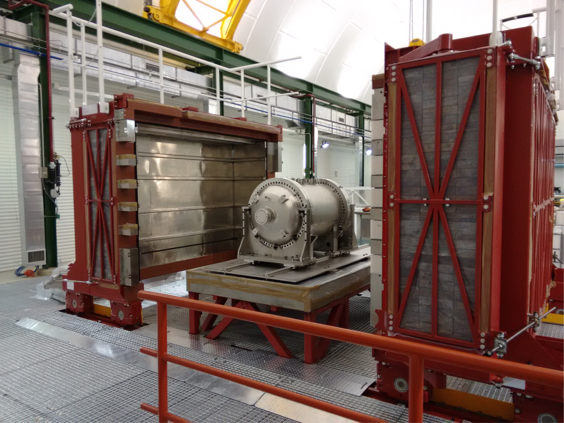
\includegraphics[width=0.9\textwidth]{img/NewCastle.png}
\caption{\small El detector NEW, instalado en el castillo de plomo que blinda el experimento de la radiación exterior.} \label{fig.NewCastle}
\end{figure} 

\begin{figure}
\centering
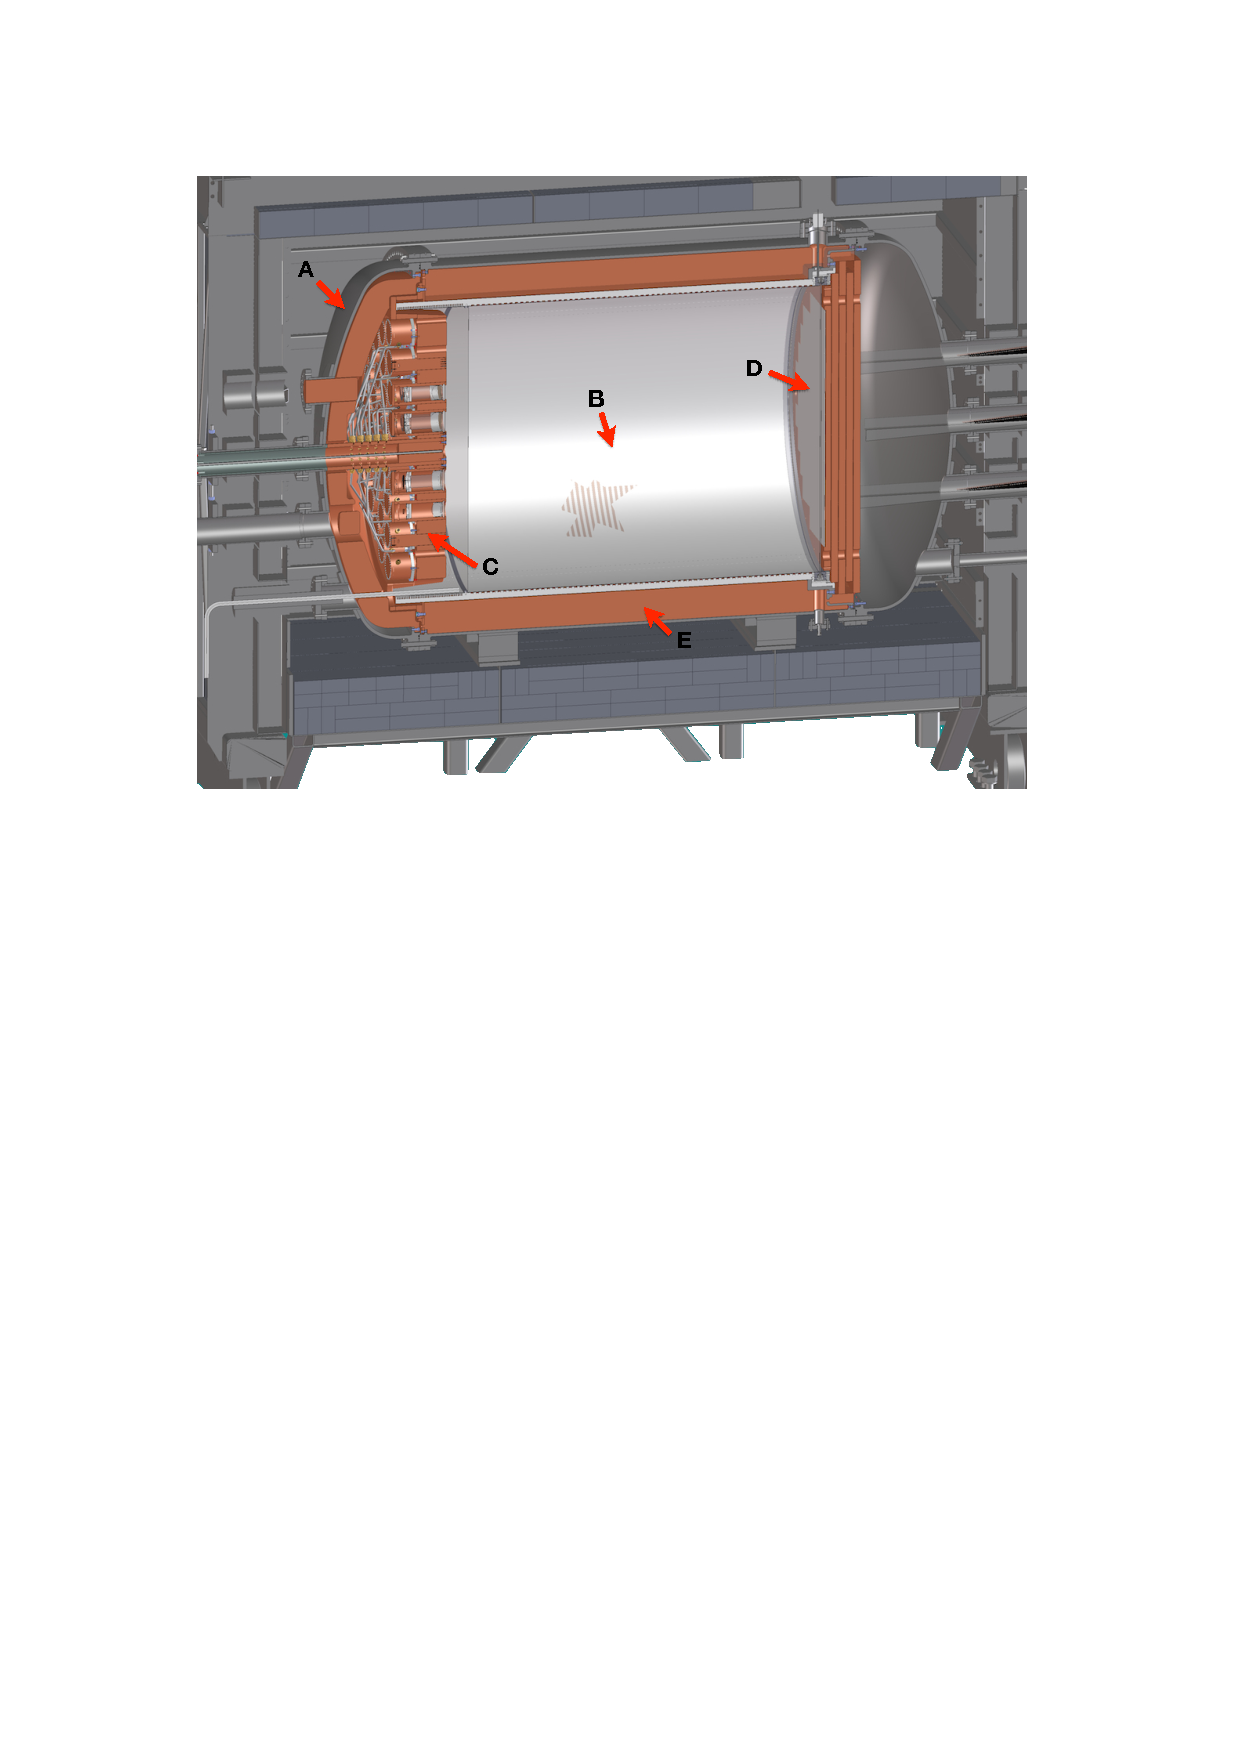
\includegraphics[width=0.9\textwidth]{img/NEXT100.pdf}
\caption{\small Sección transversal del detector NEXT-100, localizado en el interior del blindaje de plomo. Una vasija de presión hecha de acero-titanio (A) alberga la jaula eléctrica (B) y los dos planos de sensores (plano de trazado, C, plano de energía, D), localizados en los extremos de la cámara. El volumen activo está aislado de la radiación exterior por 12 cm de cobre (E).
} \label{fig.NEXT100}
\end{figure}

El experimento NEXT se ha desarrollado en varias fases. 
 \begin{enumerate}
\item Primera fase, correspondiente a I+D+i, que abarcó desde 2008 hasta 2014. Los hitos fundamentales de esta fase fueron la construcción y operación del detector NEXT-DEMO (Figura \ref{fig.DEMO}) que ha demostrado el gran potencial de la novedosa tecnología HPXe-EL en la que se basa NEXT. 
\item Segunda fase, correspondiente a la operación en el LSC del detector NEW (Figura \ref{fig:NEW}), que está siendo puesto a punto en el LSC durante 2015 (Figura \ref{fig.NewCastle}) y empezará a tomar datos en 2016. NEW operará por un periodo de 2 años (2016 y 2017) y su objetivo principal es medir los ruidos de fondo radioactivos, así como establecer y probar todas las infraestructuras necesarias (sistema de gas, sistemas automáticos de control y seguridad, sistema de blindaje, sistema de supresión de radón) para la operación de NEXT-100.
\item Tercera fase, correspondiente a  la operación en el LSC del detector NEXT-100  (Figura \ref{fig.NEXT100}). Esta fase empezará en 2018 y podría extenderse durante 3 años.
 El objetivo de NEXT-100 es alcanzar un periodo 
$\Tonu \sim 10^{26}$, explorando por tanto una región aún no estudiada, donde un descubrimiento sería posible.  Otros experimentos (GERDA-II, CUORE, KamLAND-ZEN, EXO y SNO+) intentarán también encontrar este proceso durante los próximos años, utilizando diversas técnicas e isótopos, por lo que es posible que se produzca un descubrimiento, del que NEXT podría ser parte, combinando varias técnicas e isótopos. 
\item Cuarta fase (detector NEXT2N) que podría empezar a partir de 2021, con la construcción de un detector en el rango de 300--500 kg, en el que además se reduciría el ruido de fondo específico de NEXT-100, mediante una serie de mejoras que se desarrollarán en los próximos años y que incluyen: a) sustituir los PMTs del plano de energía por SiPMs de gran área; b) introducir electrónica de digitalización en el interior de la cámara, mediante ASIC especializados; c) reducir la difusión en el xenón, mediante la adición de mezclas apropiadas (e.g, una mezcla con 0.1\% de CH$_4$~ está siendo estudiada en la actualidad); En general todas etas mejoras van en la dirección de reducir la radioactividad de los componentes de NEXT y de mejorar tanto su resolución en energía como la señal topológica. 
\end{enumerate}


\subsection*{Objetivos: NEXT}

El primer objetivo de este proyecto es contribuir de manera decisiva al desarrollo del experimento NEXT. Los objetivos específicos son los siguientes:

\subsubsection*{Operación de los detectores NEW y NEXT-100 en el LSC}

Tanto NEW como NEXT operarán de manera rutinaria durante las 24 horas del día, por un periodo de 10 meses al año (no se opera durante el mes de Agosto, ya que el LSC cierra por descanso anual y las operaciones de mantenimiento requieren unas cuatro semanas al año). Durante todo el periodo de operación es necesaria la presencia de miembros del equipo NEXT en el laboratorio. La regulación del LSC requiere que haya siempre dos personas en las instalaciones subterráneas, lo cual define el tamaño mínimo del equipo. Durante las épocas de instalación o mantenimiento, el número de físicos e ingenieros de NEXT suele ser de 6-8 personas.

La forma de operación habitual en una colaboración internacional como NEXT es repartir turnos de trabajo entre los científicos e ingenieros que integran la colaboración. No obstante, el grupo del IFIC es responsable de la coordinación de operaciones y el grupo de la UPV de la dirección organizativa (project management). La operación de los detectores requiere la presencia en el LSC del coordinador de operaciones (IFIC) y, con mucha frecuencia del Project Manager (UPV) y del coordinador técnico (IFIC). 

\subsubsection*{Análisis de datos de los detectores NEW y NEXT-100} 

Durante 2016 y 2017 el análisis de los datos del detector NEW permitirá una detallada caracterización de los parámetros operativos de NEXT (resolución en energía, señal topológica) así como de los principales ruidos de fondo. Durante 2018 y 2019 el análisis de los datos de NEXT-100 se centrará en la búsqueda de procesos \bbonu. El grupo del IFIC incluye el coordinador de software y el coordinador de análisis, que lideran estas actividades. 

Entre los trabajos a realizar en la fase NEW se cuentan: i) la calibración de los detectores con fuentes radiactivas (\ensuremath{^{83}}Kr, \NA, \CS, etc.); ii) la medida de la resolución en energía y su dependencia con la energía de operación; c) el estudio detallado de la señal topológica; d) el estudio detallado del impacto de los ruidos de fondo, en particular de las emanaciones internas de radón. Durante la fase NEXT-100 se procederá a la búsqueda de sucesos \bb\ y de sucesos \bbonu, utilizando varios análisis independientes, tanto en técnicas de filtrado (análisis convencional en el que la señal se selecciona estableciendo cortes de selección en diversas variables frente a análisis en los que se aplican técnicas de multi-variaciones o redes neuronales) como en los equipos que los llevan a cabo. El grupo del IFIC tendrá un papel de líder en la mayoría de estas actividades. 
 
\subsubsection*{Mejora de la electrónica de NEXT}

Tanto NEW como NEXT-100 operan con electrónica COTS
(de las siglas en inglés {\em commercial of the shelf}, esto es electrónica comercial disponible en el mercado) que ha sido desarrollada por el grupo de la UPV. Pese a su alta fiabilidad y buen rendimiento, la solución actual presenta algunos problemas que podrían mejorarse en el detector NEXT-100. En particular, las señales de los SiPMs y los PMTs son digitalizadas fuera de la cámara y por tanto es necesario extraerlas mediante cables de considerable longitud (del orden de 10 metros), hasta los convertidores analógico-digitales (ADCs) situados en el exterior del blindaje del detector. En el caso de NEW, se precisa, por tanto, extraer 25 cables planos (uno por KDB), a través de pasamuros diseñados para resistir la presión de operación (15 atmósferas) y para minimizar las fugas de xenón a través de ellos hasta niveles inferiores a 1 gramo por año. En el caso de NEXT-100 se precisará extraer más de 100 cables. 

El uso de electrónica COTS resulta mucho más complejo aún para la cuarta fase de NEXT, ya que se prevé que el detector NEXT2N sea un detector simétrico (SiPMs tanto en el plano de energía como en el plano de trazado) con masa en el rango de 300 a 500 kg. El número  de cables (y por tanto de pasamuros), si se opta por la misma solución adoptada por NEW y NEXT-100, sería del orden de 500. 

Una alternativa muy interesante para NEXT2N sería digitalizar la señal en el interior de la cámara, mediante ASICs especializados y extraer la señal digital, serializada, mediante fibra óptica. Esta solución, propuesta recientemente por el grupo de la UPV, minimizaría el número de pasamuros y permitiría reducir costes.

Por otra parte, como se comenta más tarde, existe la posibilidad de utilizar el mismo ASIC que se propone para el aparato PETALO como ASIC para el plano de trazado de NEXT. Además, el ASIC que se propone es un producto comercial ya existente y con un precio muy competitivo. Demostrar la viabilidad de esta solución es un importantísimo objetivo par el futuro del experimento. 


\subsection*{Desarrollo del proyecto}
Las actividades a realizar en el proyecto NEXT durante los próximos cuatro años son:
\begin{enumerate}
\item {\bf 2016}: operación del detector NEW. Calibración, estabilidad, control de riesgos (slow control), puesta a punto de la electrónica, medida de la resolución en energía y señal topológica.
\item {\bf 2017}: Medida de ruidos de fondo con el detector NEW y caracterización del modelo de ruido de fondo para NEXT. 
\item {\bf 2018}: Construcción y puesta a punto del detector NEXT-100. 
\item {\bf 2019}: Operación del detector NEXT-100. Búsqueda de señales \bbonu.  Sustitución de la electrónica del plano de trazado de NEW con electrónica ASIC para demostrar la viabilidad de esta solución para NEXT2N. 


\end{enumerate}

\subsection*{Financiación del proyecto}

La fase de I+D+i del experimento NEXT fue financiada por un proyecto CONSOLIDER-INGENIO, llamado CUP. Durante esta fase se construyó y operó el detector NEXT-DEMO. La construcción  detector NEW, así como del detector NEXT-100 cuentan con la financiación de un AdG/ERC y un proyecto coordinado de la convocatoria RETOS 2014. La financiación existente, sin embargo, no cubre todas las necesidades de personal y de operación del experimento. En este proyecto se solicita financiación para contribuir a la operación de NEW, así como para un contrato de ingeniero compartido con el proyecto PETALO, como se detalla más adelante. También se solicita financiación para demostrar la viabilidad de una electrónica digital en el interior de la cámara, para lo cual se propone sustituir la electrónica del plano de trazado de NEW con electrónica ASIC. 



\section*{Proyecto PETALO}


\subsection*{Aparatos PET}

 Una de las aplicaciones más importantes de la tecnología de detectores de física nuclear y de partículas a la imagen médica son los llamados aparatos PET, de las siglas en inglés Tomografía de Emisión de Positrones. Su principio de operación se basa en inyectar en el paciente un radiofármaco emisor de positrones, tal como la Fluordesoxiglucosa (18FDG), un azúcar radioactivo en el que un átomo de oxígeno se sustituye por uno de fluor-18 (\ensuremath{^{18}}F). El 18FDG se concentra en aquellas zonas del paciente que consumen elevadas cantidades de glucosa y por lo tanto puede actuar como trazador de procesos oncológicos (ya que las células tumorales son ávidas consumidoras de glucosa) así como de zonas del organismo con gran actividad metabólica, tales como el cerebro. El \ensuremath{^{18}}F se desintegra emitiendo un positrón, el cual se aniquila, tras un corto recorrido, con un electrón del tejido del paciente produciendo dos fotones de 511 kilo electrón voltios (keV) que se emiten en direcciones opuestas. 


%\begin{figure}
%\centering
\begin{center} \figbox[label={fig.PET}]{{\small Principio de operación del PET.}}{
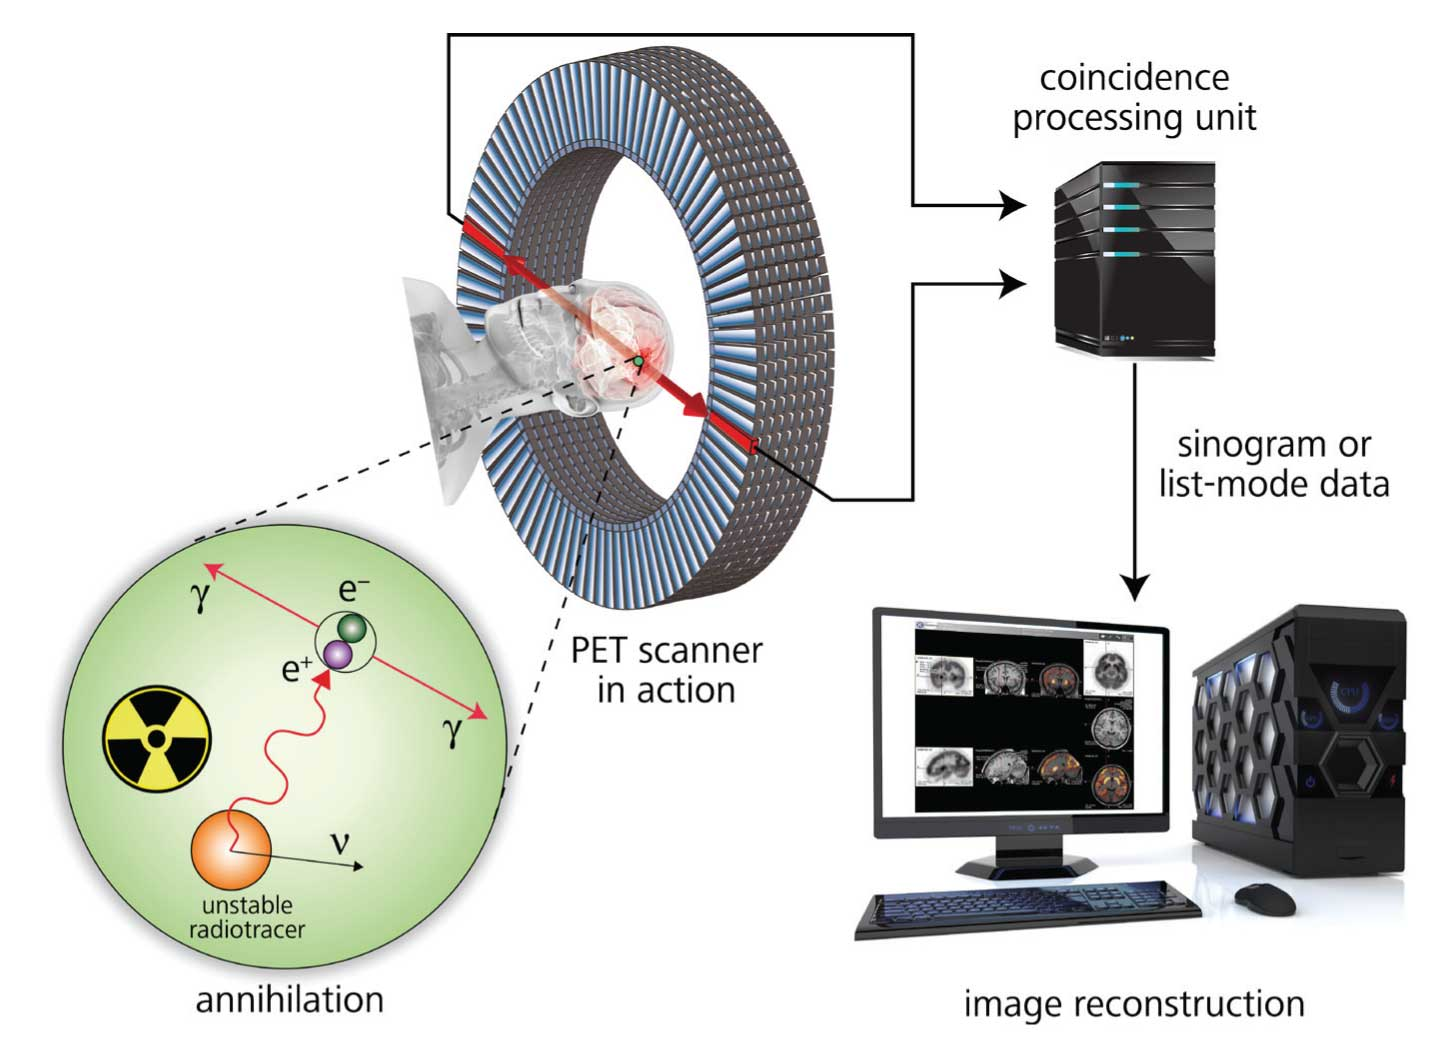
\includegraphics[width=0.6\textwidth]{img/PET.jpg}
%\caption{\small Principio de operación del PET.}
%\label{fig.PET}
} \end{center} 


Un PET clínico se construye a partir de varios anillos de detectores que rodean una determinada zona del cuerpo del paciente. Los fotones de 511 keV interaccionan con los detectores que forman el anillo, depositando su energía en ellos. Los detectores reconstruyen tanto la energía de los fotones originales como su punto de impacto. Puesto que los fotones se emiten en direcciones opuestas, cuando un par de detectores enfrentado entre sí en el anillo detectan interacciones simultáneas (dentro de la resolución temporal del sistema), pueden utilizarse los dos puntos de impacto reconstruidos para trazar una línea recta (o LOR, de las siglas en inglés de Línea de Respuesta) que pasa por el punto donde se aniquila el positrón con el electrón (el cual a su vez está muy próximo al punto de emisión del positrón). La intersección de muchas de estas LOR permite la reconstrucción funcional de la imagen (esto es, la reconstrucción de la zona en términos de su actividad metabólica), tal como se ilustra en la Figura \ref{fig.PET}.

El concepto de PET fue introducido a finales de la década de 1950 y la investigación básica que llevó a su implantación como aparato de imagen médica se ha seguido desarrollando a lo largo de las últimas seis décadas. Los aparatos PET de diseño moderno, basados en múltiples anillos de detectores, se desarrollan a partir de la década de 1990 y con mayor importancia a partir de los primeros años de la década de los 2000. Los aparatos originales utilizaban cristales ioduro de sodio (NaI) como material centelleador y PMTs como detectores de la luz visible emitida por estos cristales como respuesta a la interacción de los fotones de 511 keV. Durante los últimos cinco años, el campo ha experimentado una transformación importante, prefiriéndose en la actualidad los detectores de LSO o LYSO (de las siglas en inglés de Lutetium oxyorthosilicate o Lutetium-yttrium oxyorthosilicate) y un nuevo tipo de fotosensores llamados fotomultiplicadores de silicio (SiPMs de sus siglas en inglés). 

Los modernos aparatos PET basados en LYSO y SiPMs presentan muchas ventajas. El LYSO es un material muy denso (7.4 g/cm$^3$) capaz de detener a los fotones de 511 keV con una longitud de atenuación típica de 11 mm. Se trata además de un excelente centelleador que emite unos 14,000 fotones de luz azul (con un pico a 428 nm) por cada fotón de 511 keV absorbido. La copiosa emisión de luz se traduce a su vez en buena resolución en energía (del orden de 10-15 \% FWHM) y buena resolución espacial en la reconstrucción de las coordenadas transversas (con respecto a la dirección de vuelo) del punto de impacto (del orden de 1-3 mm) El tiempo de emisión es rápido, con una constante de atenuación de 40 ns, lo que permite una buena resolución en la coincidencia temporal (CRT de sus siglas en inglés) del orden de varios centenares de picosegundos en los sistemas comerciales más avanzados disponibles en la actualidad, tales como el GEMINI de Philips\footnote{http://www.healthcare.philips.com/main/products/nuclearmedicine/products/geminitf/}. Reducir el CRT tanto como sea posible es uno de los objetivos más importantes de la investigación actual en PET, ya que un CRT suficientemente bueno permite una mejora espectacular en la sensibilidad del sistema (la sensibilidad mide la calidad de la imagen que puede obtenerse por unidad de dosis absorbida en el paciente).  De hecho, la sensibilidad efectiva de un sistema PET para reconstruir un objeto de radio D mejora como D/CRT. 

Por otra parte, los sistemas basados en LYSO tienen algunos inconvenientes importantes. El mayor es el elevado precio de estos cristales, que a su vez constituye casi la mitad del coste del sistema PET. Un aparato comercial basado en LYSO puede costar hoy en día varios millones de euros. Este elevado coste, comparado con otras técnicas (tomografía axial, por ejemplo) limita el rango de aplicación del PET a la imagen médica. Por otra parte, las aplicaciones TOF de sistemas basados en LYSO, aunque posibles, están limitadas por la velocidad de centelleo intrínseca del centelleador (40 ns), el elevado índice de refracción (1.8)  y el hecho de que estos sistemas no miden en general la coordenada longitudinal (a lo largo de la línea de vuelo del fotón de 511 keV). Por tanto no se dispone de la medida de la profundidad de la interacción (DOI de sus siglas en inglés), lo que también limita la precisión en TOF. A pesar de estas limitaciones, el desarrollo de aparatos comerciales como el GEMINI de Philips, capaz de explotar la técnica TOF para mejorar su sensibilidad, a pesar de un modesto CRT (del orden de 500-600 ps), pone de manifiesto el extraordinario potencial de la tecnología.

\subsection*{Aplicación de la tecnología de Xenon Líquido a PET}

La posibilidad de construir un detector PET basado en el xenón líquido (LXe) fue propuesta por Chepel en 1973\footnote{Chepel, V.Y., 1993, Nucl. Tracks Radiat. Meas. 21, 47.}  pero la I+D+i subsiguiente se encontró con problemas tecnológicos que han limitado hasta la actualidad el desarrollo de este tipo de detectores\footnote{F. Nishikido et al. J. Appl. Phys. 43, 779 (2004).}. En concreto, la posibilidad de desarrollar un PET basado únicamente en la medida de la luz de centelleo del xenón fue estudiado hace una década por el grupo de Waseda, que obtuvo resultados modestos asociados a limitaciones tecnológicas, en concreto el uso de PMTs que a su vez limitaba la homogeneidad y hermeticidad de la celda de detección. 

No obstante, las propiedades físicas del LXe le permiten competir con ventaja con los mejores detectores de centelleo sólido, tales como el LYSO. Concretamente, el LXe produce el doble de luz (30,000 fotones) por fotón de 511 keV absorbido que el LYSO y una fracción importante de estos fotones (del orden de 6,000) se emiten con una constante de decaimiento muy rápida (2.2 ns). Por otra parte, la resolución temporal intrínseca de un sistema viene determinada por el número de fotones sobre la constante de decaimiento (N/$\tau$). N$/\tau$ =2,727 para la constante rápida ($\tau$ = 2.2~ ns) del LXe a comparar con N/$\tau$ =333 para el LYSO ($\tau$ = 40~ ns). Por tanto, el LXe proporciona, a priori, un CRT ocho veces mejor que el del LYSO. Pero además un detector basado en el LXe puede medir con precisión del orden de 1 mm las 3 coordenadas del punto de interacción del fotón incidente, mientras que la resolución en el DOI suele estar limitada en LYSO a varios milímetros. Por otra parte, la corrección en el tiempo de vuelo del fotón desde que se emite hasta que alcanza el fotodetector es importante (en el caso del LYSO esta corrección es aún más importante que en el LXe debido a su alto índice de refracción, 1.8 a comparar con 1.55), lo que implica una mayor degradación del CRT en LYSO comparado con LXe. Como consecuencia, el LXe ofrece la posibilidad de construir un detector PET con una resolución CRT muy superior a la del LYSO. La resolución intrínseca de la celda centelleadora de xenón líquido, LXSC  se ha calculado en 20 ps\footnote{J.J. Gómez-Cadenas, charla plenaria en la conferencia CSI 2015, artículo en preparación (proceedings, CSI 2015). }  lo que permite la posibilidad de construir sistemas comerciales con un CRT un orden de magnitud mejor de los que obtiene el sistema GEMINI. Un sistema de este tipo supondría una auténtica revolución en la tecnología PET.

La segunda característica de interés del LXe es su bajo coste, del orden de un factor 5 inferior (por unidad de detección) al LSYO. Esto permite la posibilidad de construir un PET que conjunte una sensibilidad muy superior a los modelos convencionales (gracias a la aplicación TOF) con un coste sensiblemente inferior. 

%\begin{figure}
%\centering
\begin{center} \figbox[label={fig.BOX}]{{\small Diseño de la LXSC.}}{
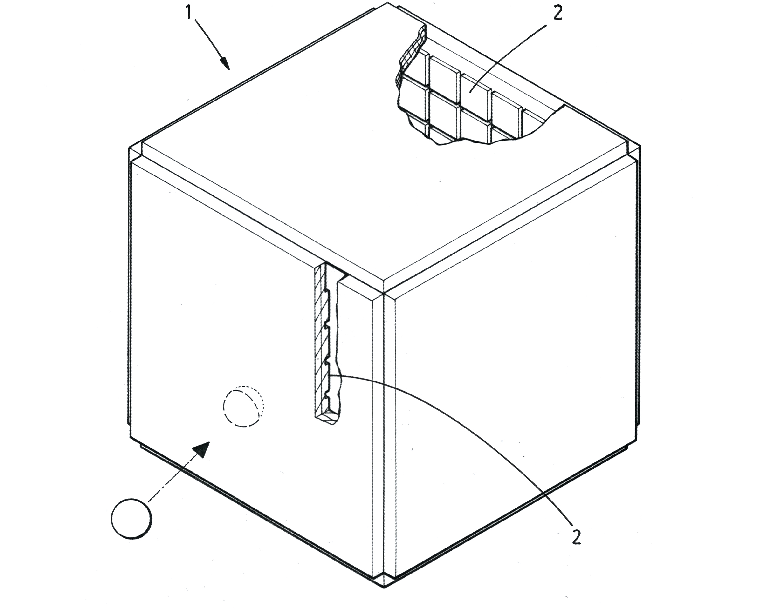
\includegraphics[width=0.6\textwidth]{img/LXSC2.pdf}
%\caption{\small Diseño de la LXSC.}
%\label{fig.BOX}
} \end{center} 

Por otra parte, la propuesta, la celda centelladora de xenón líquido (LXSC)\footnote{Celda centelleadora de LXe, patente número P201531239 presentada en 31 agosto 2015 ante la OPEM (MINECO), CSIC/UV, inventor J.J. Gómez-Cadenas.} resuelve los problemas tecnológicos encontrados por los pioneros de esta técnica, tales como el grupo de Waseda. El modelo estándar de LXSC es una caja de $5\times 5 \times 5$~ cm$^3$ (las dimensiones y la forma pueden variar dependiendo de la aplicación) rellena de LXe (Figura \ref{fig.BOX}). Cuatro de las 6 superficies internas de la LXSC están recubiertas por una lámina de teflón que refleja con 95\% de eficiencia la luz UV (172 nm) emitida por el xenón. La cara de entrada y salida (con respecto a la dirección de vuelo de los fotones) están recubiertas por SiPMs sensibles a la luz UV (fabricados en la actualidad por Hamamatsu y a cuyo desarrollo han contribuido de forma muy importante miembros del GI). El tamaño de los SiPMs puede ajustarse según la aplicación y el coste del dispositivo, variando típicamente entre 3 mm y 6 mm de lado. La LXSC ofrece una buena resolución en energía (del orden del 12 \% FWHM), buena resolución espacial (1 mm) en las tres coordenadas y excelente CRT\footnote{J.M. Benlloch Rodríguez, tesis de Master, Universidad de Valencia, 2015, dirigida por J.J. Gómez-Cadenas. 
}. {\bf Es posible, por lo tanto, construir en la comunidad valenciana un nuevo tipo de sistema PET basado en la LXSC que suponga, a la vez, una mejora en las prestaciones y una reducción del coste, relativo a los sistemas actuales.}
\subsection*{Objetivos: PETALO}

El segundo objetivo de este proyecto es realizar contribuciones esenciales para el desarrollo del proyecto PETALO, necesarias para demostrar su viabilidad y para evaluar sus capacidades. Los objetivos específicos son los siguientes: i) medida de ciertas propiedades físicas del LXe, cruciales para aplicaciones PET;  ii) caracterización de la resolución de energía y la resolución espacial de la LXSC; medida de la resolución de coincidencia temporal (CRT de sus siglas en inglés) de la LXSC.

\subsubsection*{Medida de las propiedades físicas de LXe}
La resolución en energía, resolución espacial y CRT del LXe depende de la cantidad total de fotones de centelleo ultravioleta (UV) producidos como respuesta a los fotones de 511 keV característicos del PET. Depende también de la fracción de la energía depositada que resulta en centelleo y en ionización. Son necesarias, por tanto, las siguientes medidas:
\begin{itemize}
\item El número total de fotones UV producidos como respuesta a fotones de 511 keV. 
\item Fracción de fotones UV debida a centelleo primario y fracción debida a la recombinación lenta de los electrones de ionización. 
\item Fracción de fotones UV debida al modo singlete y su constante de centelleo.
\item Fracción de fotones UV debida al modo triplete y su constante de centelleo. 
\end{itemize}

\subsubsection*{Medida de la resolución en energía y resolución espacial de la LXSC}

La resolución en energía de un detector de centelleo de xenón líquido es una combinación de varios factores, a saber: factor debido a la geometría del detector R$_g$, debido a la fluctuación estadística de los fotoelectrones en los sensores R$_s$, y fluctuación intrínseca, R$_i$, debida a las fluctuaciones que introducen los electrones que no se recombinan y la no proporcionalidad de la luz de centelleo:

\begin{equation}
\mathrm{R}^2 = \mathrm{R}_g^2 + \mathrm{R}_s^2 +  \mathrm{R}_i^2
\end{equation}

Este proyecto propone una medida experimental de R. La contribución de 
R$_g$~y R$_s$~se puede obtener mediante un cálculo Monte Carlo y a partir de ahí determinar la contribución intrínseca. Se espera obtener una resolución de 12\% FWHM competitiva con la de centelladores como LSO/LYSO. 

La resolución espacial en las coordenadas (x,y) se obtendrá a partir de algoritmos de baricentro que pesan la posición de los SiPMs con la amplitud del pulso. La resolución en la coordenada longitudinal se obtendrá a partir del cociente entre la amplitud total registrada en el plano de entrada y en el de salida. Se espera obtener una resolución del orden de 1--2 mm FWHM en las tres coordenadas.     

\subsubsection*{Medida de la resolución temporal de la LXSC}

La resolución temporal (CRT) de la LXSC depende de dos factores: a) la resolución temporal asociada con el disparo (trigger) de una interacción en una LXSC y b) la fluctuación temporal introducida por la sincronización de diferentes celdas.

La resolución temporal asociada a una LXSC o resolución intrínseca del sistema (ya que la resolución de sincronización, puede, en principio, reducirse arbitrariamente mediante la electrónica adecuada) depende a su vez de varios factores, a saber: el cociente $N/\tau$, donde $N$~es el número de photons emitidos con una constante temporal dada $\tau$; b) la corrección longitudinal o corrección de profundidad de interacción (DOI) que toma en cuenta el hecho de que no todas las interacciones ocurren en el mismo punto; c) la función de respuesta a fotones (PDE) de los SiPM; d) la fluctuación temporal introducida por los SiPMs y su electrónica asociada. 

El número esperado de fotones en LXe con una constante rápida (2.2 ns) es del orden de 6,000, por tanto  $N\tau$ = 6,000/2.2 = 2,727, a comparar con el correspondiente número para LSO $N\tau$ = 14,000/40 = 35. Por tanto, la CRT intrínseca del LXe es mucho mejor que la del LSO.  Nuestros estudios preliminares sugieren la posibilidad que se pretende demostrar experimentalmente, de un CRT  mejor de 100 ps, incluyendo el efecto de los SiPMs y la electrónica. 

\subsubsection*{El detector P2}

%\begin{figure}
%\centering
\begin{center} \figbox[label={fig.P2}]{{\small Esquema del detector P2.}}{
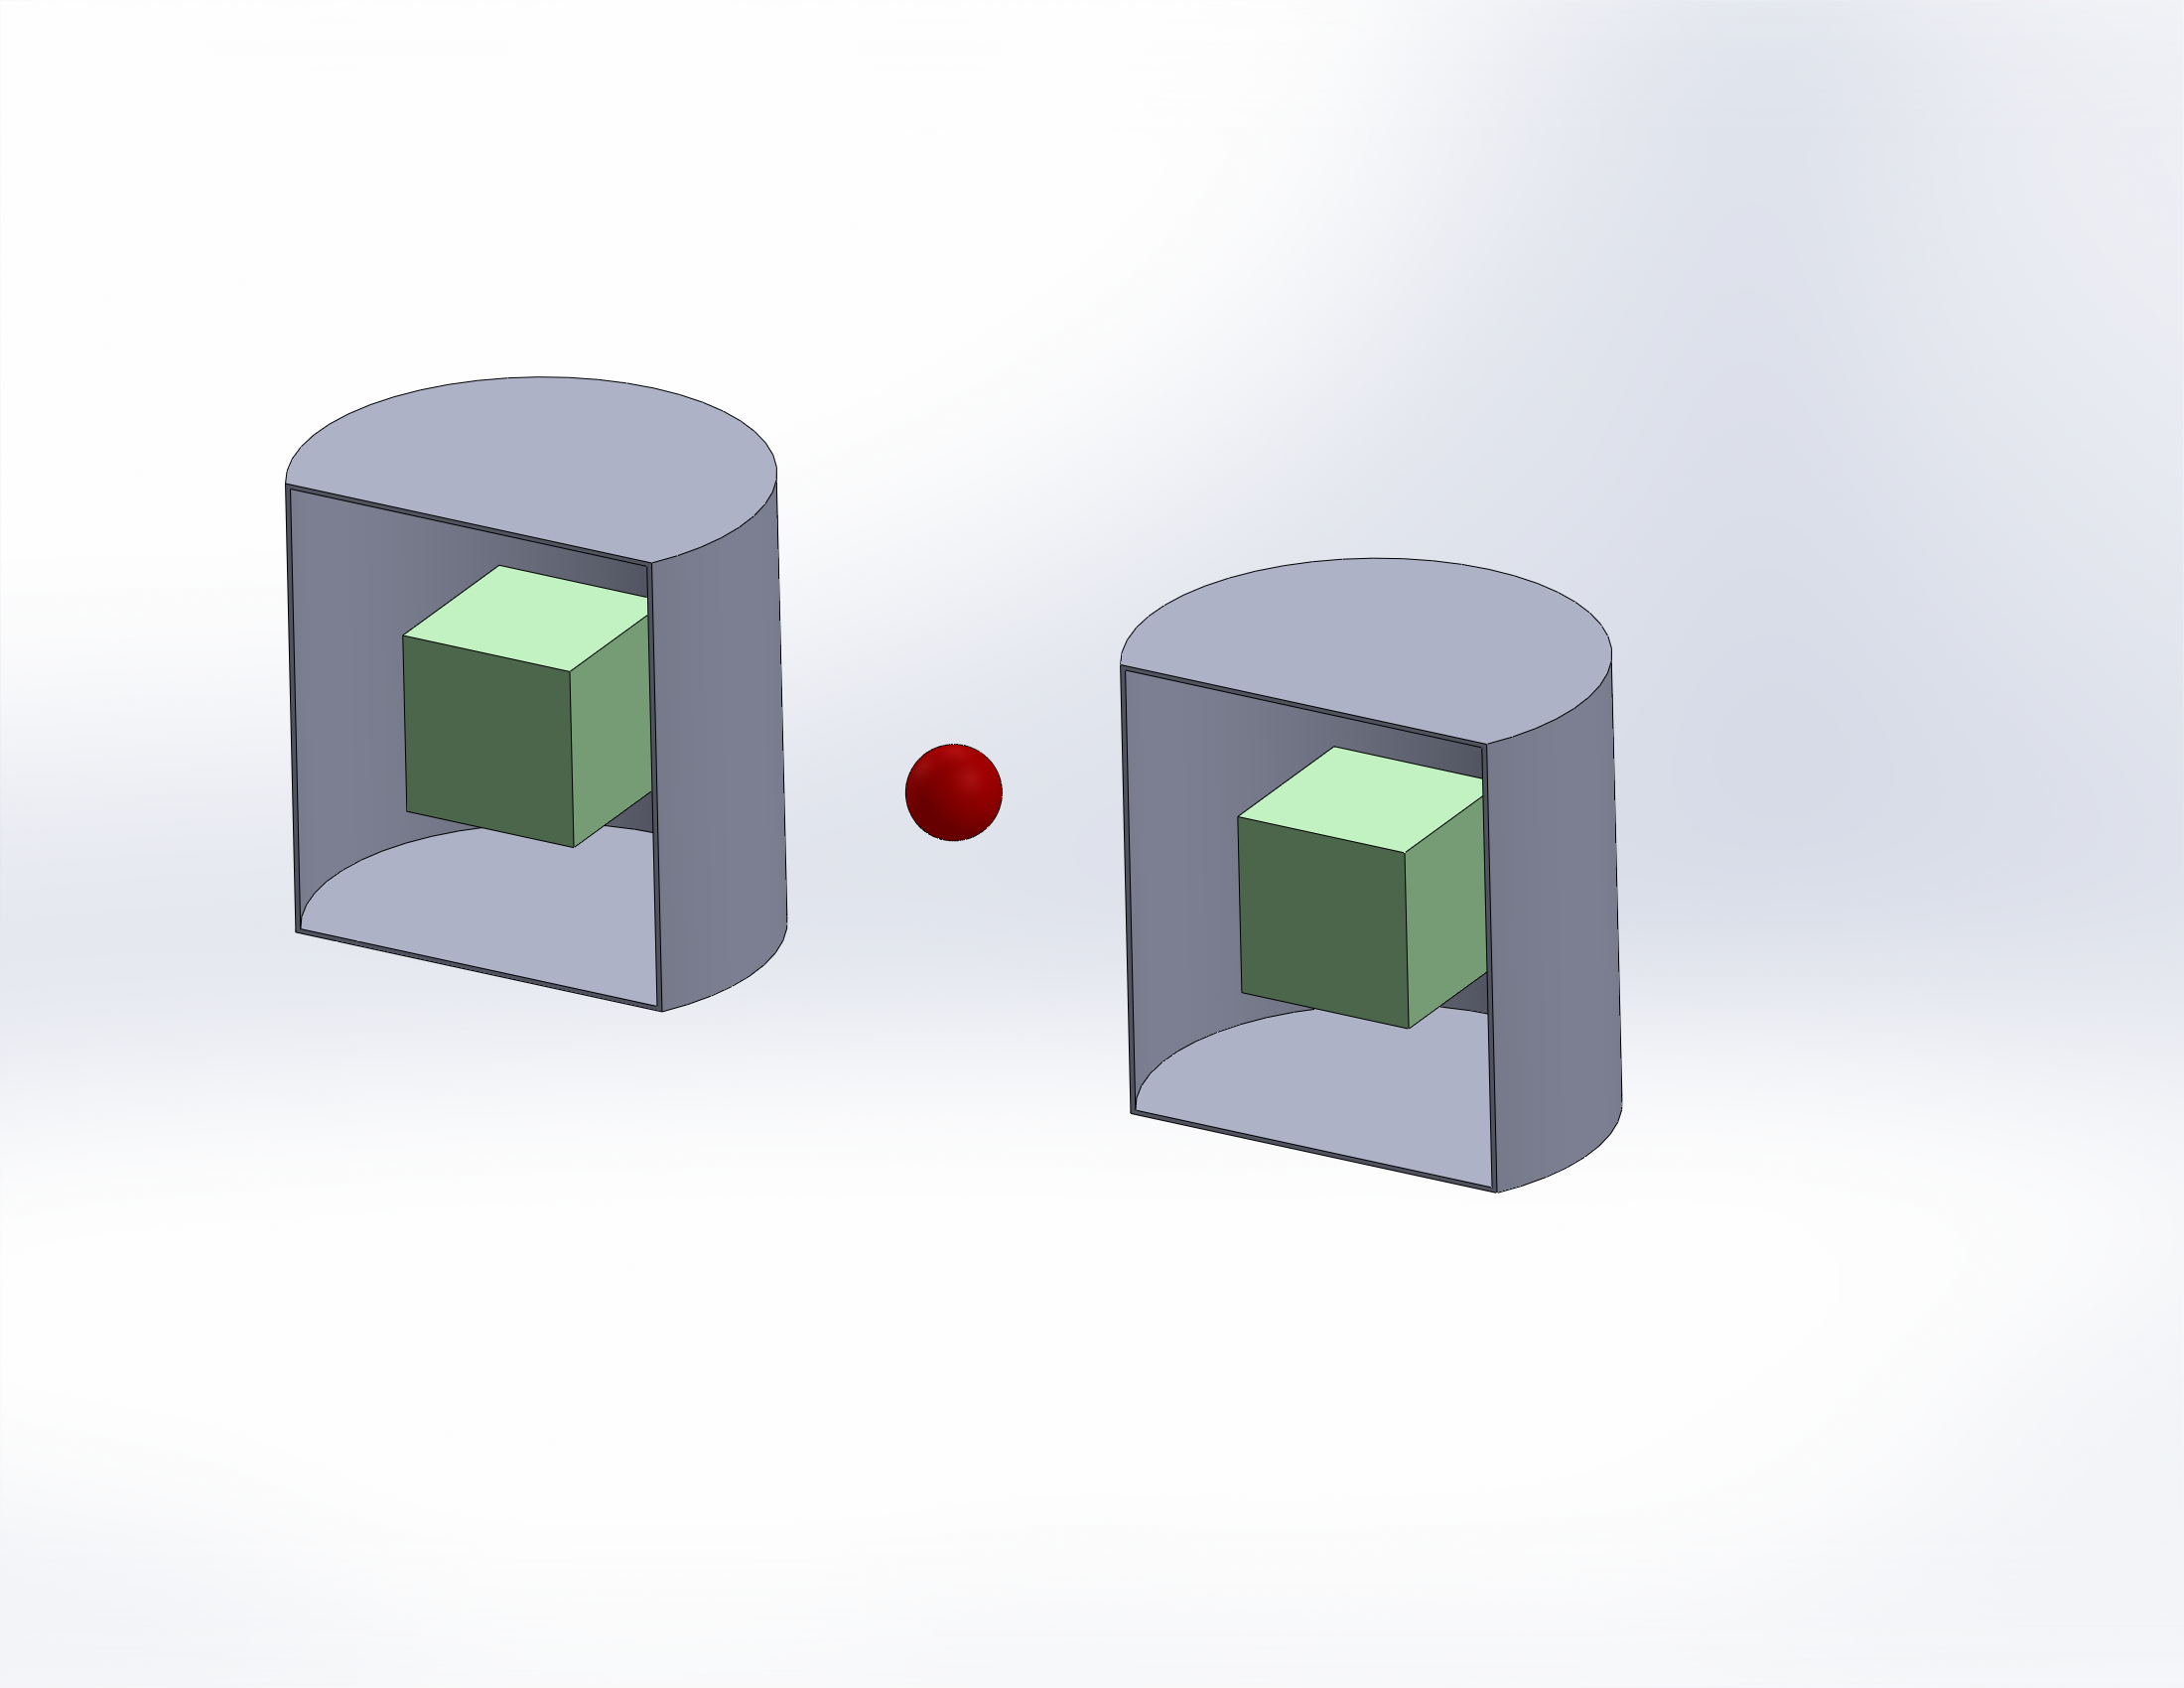
\includegraphics[width=0.6\textwidth]{img/P2.png}
%\caption{\small Esquema del detector P2.} 
%\label{fig.P2}
} \end{center}

La medida de la resolución espacial, resolución en energía y resolución CRT requiere la construcción de un sistema de test especializado que denominamos P2 (Figura \ref{fig.P2}). Se trata de dos LXSC independientes, cada una de las cuales está albergada en su propio criostato. Una de las LXSC (PA) tendrá todas las caras internas instrumentadas, a fin de poder utilizar la redundancia de las medidas de las coordenadas $(x,y)$, $(x,z)$, $(y,z)$ y la determinación independiente de la coordenada $z$~para medir la resolución en posición de la LXSC. Asímismo, la comparación de la resolución del primer fotoelectrón entre PA y la segunda LXSC (PB), que sólo tendrá dos caras instrumentadas, permitirá entender la influencia en el CRT del tiempo de tránsito de los fotones.  

\subsubsection*{Construcción y operación de un demostrador preclínico}
Una vez medidos los parámetros críticos de PETALO (resolución en energía, resolución espacial y CRT), se procederá a la construcción de un anillo constituido por catorce LXSC, que permita caracterizar la sensibilidad de un aparato PET-TOF basado en LXe. Para ello se utilizarán fantasmas estándar (NEMA phantoms) que permitirán medir los parámetros operacionales del escáner así como su fiabilidad a la hora de reconstruir imágenes.

\subsection*{Desarrollo del proyecto}
Las actividades a realizar en el proyecto PETALO durante los próximos cuatro años son:
\begin{enumerate}
\item {\bf 2016}: La construcción de un dispositivo experimental, basado en 2 LXSC cuya operación en coincidencia permite medir el CRT del sistema, así como la resolución en energía y resolución espacial de las celdas (P2).
\item {\bf 2017}: Operación de P2. Medidas de resolución y CRT. Construcción del criostato y la mecánica de un demostrador pre-clínico consistente en un anillo de 14 LXSC (PDEMO). 
\item {\bf 2018}: Construcción de los módulos de PDEMO. Puesta a punto y calibración. 
\item {\bf 2019}: Evaluación de la sensibilidad PDEMO y de su resolución TOF. Preparación de un proyecto para la construcción y comercialización de un PET-TOF de alta sensibilidad combinado con resonancia magnética (RMI) para neuroimagen cerebral.   
\end{enumerate}

\subsection*{Financiación del proyecto}

En este proyecto de investigación se solicita financiación para la construcción de P2 y de PDEMO así como para un ingeniero compartido con el proyecto NEXT. Por otra parte, el proyecto se beneficiará de la gran sinergia existente con el proyecto NEXT. En particular, PETALO utilizará el laboratorio de NEXT existente en el IFIC, así como las infraestructuras (sistema de gas, equipos de vacío, recuperación criogénica, sistema de test para SiPMs, etc.) lo que permitirá un abaratamiento muy considerable de los costes de desarrollo. 

%Sinergia entre NEXT y PETALO. 
%
%Como se ha expuesto más arriba, la tecnología que ha dado lugar al proyecto PETALO se ha derivado de la experiencia adquirida por el IP y el grupo de investigación en el desarrollo del proyecto NEXT. Concretamente, la celda centelladora de xenón líquido, LXSC, se instrumenta utilizando los KDBs desarrollados para NEXT.
%
%Un aspecto donde la sinergia entre ambos proyectos revierte desde PETALO hasta NEXT es la electrónica del plano de lectura. En el diseño original de NEXT, implementado en los detectores NEXT-DEMO y NEW, se utiliza electrónica discreta disponible comercialmente (COTS, de sus siglas en inglés). Dicha electrónica es fiable y proporciona una excelente respuesta, pero resulta muy cara, con un coste del orden de 150 euros por canal. De hecho, la electrónica del plano de trazado de NEXT-100 se presupuestó en cerca de 1 millón de euros. Dado lo ajustado de la financiación para el proyecto NEXT, reducir este coste es esencial para poder construir el detector final. 
%
%Por otra parte, ningún sistema PET que aspire a implantarse comercialmente puede permitirse electrónica COTS, dado su alto precio. La solución, sin embargo, ya ha existe en el ámbito PET, con el desarrollo de varios ASIC especializados para leer SiPMs, entre los que cabe destacar el TOFPET y TOFPET2 de PETSYS . Cada ASIC cuenta con 64 canales (por tanto puede adaptarse a un KDB) y su coste de producción es del orden de 20 € por canal. 
%
%Durante 2016, el proyecto PETALO pondrá en marcha el demostrador P2, utilizando el TOFPET, cuya resolución temporal es excelente. Como consecuencia, es posible certificar, en 2017, la viabilidad de una electrónica basada en ASIC (en lugar de en COTS) no sólo para PETALO, sino también para NEXT-100. Esta solución permitiría reducir el coste de la electrónica de NEXT-100 desde casi un millón de euros hasta 140,000 euros, lo que supondría un ahorro esencial para el proyecto. 
%
%
%
%
%
%
%



























\end{tcolorbox}

\newpage

\begin{tcolorbox}[breakable,colback=white,coltitle=black,arc=0pt,outer arc=0pt,colframe=black,boxrule=0.6pt,boxsep=0pt,left=0pt,top=0pt,right=0pt]
{\bf
Justificació del pressupost del projecte d’investigació, per a tota la durada del projecte, distribuït per anualitats
Justificación del presupuesto del proyecto de investigación, para toda la duración del proyecto, distribuido por anualidades
}

La operación de los detectores NEW y NEXT-100 en el LSC requiere la presencia continuada de un equipo de científicos en Canfranc. En concreto, el IFIC es responsable de la coordinación de operación y técnica, mientras que la UPV es responsable de la coordinación de proyecto. Esto implica la presencia del coordinador de operaciones y el coordinador de proyecto durante 5 meses al año cada uno (normalmente ambos coordinadores alternan su presencia en el LSC). 

Los gastos de manutención (promediados durante periodos largos) se estiman en 2,000 euros por persona y mes. Por tanto, los gastos de operación para NEXT se estiman en 20,000 euros al año (dos personas durante 5 meses por año). 

El punto de sinergia más claro entre el proyecto NEXT y el proyecto PETALO es la electrónica. Los detectores P2 y PDEMO requieren ASIC especializados para medir el tiempo de vuelto. En concreto, se planea utilizar el 
TOFPET2 ASIC fabricado por PETSYS\footnote{\url{http://www.petsyselectronics.com/web/website/docs/products/product1/Flyer\%20ASIC\%20TOFPETv2.pdf}}. Se trata de un nuevo chip, con 64 canales, especialmente diseñado para aplicaciones TOF. Sus características le hacen ideal para su uso en P2 y PDEMO, {\bf pero además este ASIC podría sustituir a la electrónica COTS de NEXT}, de cara a una cuarta fase del proyecto. 

En consecuencia, se solicita financiación para un ingeniero electrónico durante los cuatro años del proyecto (coste estimado 40,000 euros al año) cuya actividad principal estará relacionada con la implementación de las soluciones ASIC tanto para PETALO como para NEXT. Además, este ingeniero jugará un rol decisivo en la puesta a punto de P2 (puesta a punto de SiPMs, adquisición de datos, etc.), así como en la mejora del plano de trazado de NEW utilizando la electrónica ASIC. 

El detector P2 se construirá en 2016. Su coste se estima en 30,000 \euro. P2 requiere la construcción de dos pequeños criostatos para albergar de manera independiente las dos LXSC que utilizará el sistema (coste estimado de los dos criostatos y la mecánica asociada 15,000 \euro). El coste del módulo PB (2 caras instrumentadas) se estima en 2,500 \euro. El coste del módulo PA (6 caras instrumentadas) se estima en 7,500 \euro. El coste total de PA y PB es 10,000 \euro. Se estiman en 5,000 \euro\ los gastos asociados a infraestructuras, fuente radioactiva, etc. 

En 2017 se construirá el criostato de PDEMO, diseñado para albergar un anillo de 14 módulos y cuyo coste se estima en 20,000 \euro. Se prevén además 10,000 \euro\ para construir los primeros 4 módulos de PDEMO.

En 2018 se construirán los diez módulos restantes de PDEMO (25,000 \euro). Se prevén 5,000 \euro\ para la adquisición de dispositivos de prueba para PDEMO (fantasmas NEMA). 

En 2019 se prevén 30,000 \euro\ para la mejora de 1,600 canales de electrónica en el plano de trazado de NEW. Se prevé un coste de 20,000 \euro\ para los ASIC y 10,000 \euro\ para la infraestructura asociada (fibra óptica, pasamuro para fibra óptica, módulos externos, etc.).

En resumen, el gasto puede desglosarse, de manera uniforme, durante los cuatro años del proyecto de la siguiente manera:
\begin{enumerate}
\item {\bf Personal}. Un ingeniero compartido entre NEXT y PETALO (40,000 \euro\ año).
\item {\bf Viajes y alojamiento}. Operación de NEXT en el LSC, 2 personas, a 5 meses por persona y 2,000 \euro\ al mes para manutención, alojamiento y viaje (20,000 \euro\ año).
\item {\bf Fungible}. Construcción de P2, PDEMO y mejora de la electrónica de NEXT (40,000 \euro).

\end{enumerate}


\end{tcolorbox}

\newpage

\begin{tcolorbox}[breakable,colback=white,coltitle=black,arc=0pt,outer
  arc=0pt,colframe=black,boxrule=0.6pt,boxsep=0pt,left=0pt,top=0pt,right=0pt]

{\bf Membres de l'equip de treball i tasques a desenrotllar 
Miembros del equipo de trabajo y tareas  a desarrollar }

El equipo de investigación incluye: 

\begin{enumerate}
\item Prof. J.J. Gómez-Cadenas, PI CSIC, CU UV (excedente). Es el investigador principal (PI) del proyecto. 
\item Prof. F. Mora (CU, UPV, I3M), cuya tarea es la supervisión del desarrollo de la electrónica ASIC para PETALO y NEXT.
\item Prof. J. Díaz (CU, IFIC), cuya tarea es la supervisión del desarrollo del proyecto PETALO. El profesor Díaz es el IP del proyecto solicitado a RETOS-2015 para el desarrollo de PETALO. 
\item Prof. J. Toledo (TU, UPV, I3M), cuya tarea es actuar como coordinador de proyecto (Project Manager) de NEXT y PETALO.
\item Prof. R. Esteve (TU, UPV, I3M), cuya tarea es el desarrollo del DAQ para NEXT y PETALO.
\item Dr. A. Cervera (CT, CSIC, IFIC), cuya tarea es la coordinación de la reconstrucción de eventos en NEXT y reconstrucción de imagen en PETALO (los algoritmos usados en ambos casos son muy similares, ya que NEXT ha adoptado para la reconstrucción de trazas las técnicas de maximización de probabilidad típicas de imagen médica).
\end{enumerate}

El equipo de trabajo incluye:
\begin{enumerate}
\item Dr. M. Sorel (R\&C en extensión de contrato, CSIC, IFIC), cuya labor es la coordinación del programa de física de NEXT.
\item Dr. P. Novella (R\&C, CSIC, IFIC), que actuará como Software Manager de NEXT y PETALO.
\item Dra. N. Yahlali (AD, UV, IFIC), responsable de los estudios de caracterización de SiPMs para PETALO. 
\item Dr. I. Liubarsky (científico sénior contratado, CSIC, IFIC), cuya labor es la coordinación técnica de ambos proyectos.
\item Dr. A. Laing (post-doc, UV, IFIC), cuya labor es la coordinación de operación de NEW y NEXT.
\item Dra. P. Ferrario (post-doc, UV, IFIC), cuya tarea es el desarrollo de simulaciones para NEXT y PETALO. 
\item Dra. N. López-March (post-doc. UV, IFIC) cuya tarea es el análisis de datos para NEXT y PETALO.
\end{enumerate}

El grupo de investigación cuenta además con los siguientes ingenieros y estudiantes de doctorado. 
\begin{enumerate}
\item J. Rodríguez (ingeniero electrónico, CSIC, IFIC), responsable del plano de trazado de NEXT y del desarrollo de los KDBs para PETALO. 
\item V. Álvarez (ingeniero electrónico, UV, IFIC), responsable del plano de energía de NEXT.
\item M. Querol (ingeniero electrónico. UV, IFIC), responsable del desarrollo de slow-controls para NEXT y PETALO.
\item S. Cárcel (ingeniero mecánico, UV, IFIC), responsable de la mecánica de NEXT.
\item A. Martínez (ingeniero mecánico, UV, IFIC), a cargo de la mecánica para PETALO. 
\item J.V. Carrión (ingeniero informático, CSIC, IFIC), a cargo de la informática para NEXT y PETALO. 
\item Ander Simón (estudiante de doctorado, UV, IFIC). Tesis doctoral sobre el plano de trazado de NEXT y algoritmos de reconstrucción para NEXT.
\item Miquel Nebot (estudiante de doctorado, UV, IFIC). Tesis doctoral sobre el plano de energía de NEXT y estudios sobre radón.
\item J. Pérez (estudiante de doctorado, UV, IFIC). Tesis doctoral sobre medidas de las trazas radioactivas en las componentes del detector NEXT.
\item J. M. Benlloch Rodríguez (estudiante de doctorado, CSIC, IFIC). Tesis doctoral sobre PETALO.  
\end{enumerate}


























\end{tcolorbox}

\end{document}